%%%%%%%%%%%%%%%%%%%%%%%%%%%%%%%%%%%%%%%%%%%%%%%%%%%%%%%%%%%%%%%%%%%%%%%%%%%%%%%%
% IEEE RAS conference template (ieeeconf.cls, PaperCept). 6-page limit.
%%%%%%%%%%%%%%%%%%%%%%%%%%%%%%%%%%%%%%%%%%%%%%%%%%%%%%%%%%%%%%%%%%%%%%%%%%%%%%%%
\documentclass[a4paper, 10pt, conference]{ieeeconf}

\IEEEoverridecommandlockouts
\overrideIEEEmargins

\usepackage{cite}
\usepackage{amsmath,amssymb,amsfonts}
\usepackage{graphicx}
\graphicspath{{../figures/}}
\usepackage{textcomp}
\usepackage{xcolor}
\usepackage[T1]{fontenc}
\usepackage[utf8]{inputenc}
\usepackage[hyphens]{url}

\setlength{\textfloatsep}{7pt plus 1pt minus 2pt}
\setlength{\floatsep}{6pt plus 1pt minus 1pt}
\setlength{\intextsep}{6pt plus 1pt minus 1pt}

% Allow denser float packing than the LaTeX defaults (2 top / 1 bottom / 3 total)
\setcounter{topnumber}{3}
\setcounter{bottomnumber}{2}
\setcounter{totalnumber}{4}
\renewcommand{\topfraction}{0.92}
\renewcommand{\bottomfraction}{0.75}
\renewcommand{\textfraction}{0.07}
\renewcommand{\floatpagefraction}{0.80}
\AtBeginDocument{%
  \setlength{\abovedisplayskip}{3pt plus 1pt minus 1pt}%
  \setlength{\belowdisplayskip}{3pt plus 1pt minus 1pt}%
  \setlength{\abovedisplayshortskip}{2pt}%
  \setlength{\belowdisplayshortskip}{2pt}}

\title{\LARGE \bf
A Federated Expert-Fusion Framework for Cross-Bank Fraud Detection
}

\author{Shreeshailya Patil$^{1}$, Yike Li$^{1}$, Nicol\'as Ordo\~nez Chala$^{1}$,
Dinh Tan Nguyen$^{2}$ and Sai Ho Ling$^{3}$%
\thanks{All authors are with the Faculty of Engineering and Information
Technology, University of Technology Sydney, Ultimo, NSW 2007, Australia.}%
\thanks{$^{1}$S. Patil, Y. Li and N. Ordo\~nez Chala:
{\tt\small shreeshailya.patil@student.uts.edu.au},
{\tt\small yike.li-1@student.uts.edu.au},
{\tt\small nicolas.ordonezchala@student.uts.edu.au}}%
\thanks{$^{2}$D. T. Nguyen is with the School of Biomedical Engineering
{\tt\small dinhtan.nguyen@student.uts.edu.au}}%
\thanks{$^{3}$S. H. Ling is with the School of Electrical, Mechanical and
Biomedical Engineering {\tt\small steve.ling@uts.edu.au}}%
}

\begin{document}

\maketitle
\thispagestyle{empty}
\pagestyle{empty}

%%%%%%%%%%%%%%%%%%%%%%%%%%%%%%%%%%%%%%%%%%%%%%%%%%%%%%%%%%%%%%%%%%%%%%%%%%%%%%%%
\begin{abstract}
Banks cannot pool transaction data for fraud detection, so we measure what
federated learning (FL) actually delivers across simulated bank silos. We
benchmark four FL algorithms, three bank-local tree experts and four
expert-fusion gates on three public fraud datasets under Dirichlet non-IID
splits ($\alpha \in \{0.05, 0.10, 0.50\}$) and five seeds: 516 runs, every
partition reproducible from (seed, dataset, $\alpha$) alone. Three findings
stand out. First, the deployable fusion gates hold the best mean rank of any
family and beat the FL family average on all three datasets (Wilcoxon
$p \le 0.030$), yet never beat the per-cell best backbone ($p \ge 0.76$): fusion
buys robustness against selecting a poor backbone, not raw accuracy. Second, FL
collapse at extreme skew is a partition sensitivity rather than an algorithm
ranking, and personalised FL never records F1 = 0. Third, a cost-aware triage
layer turns rankings into decisions: at recall 80 it auto-clears 74 to 99.8\% of
transactions, defers 4 to 5\% to human review, and its expected cost moves under
4\% while the assumed cost ratio varies fiftyfold.
\end{abstract}

\begin{keywords}
federated learning, fraud detection, expert fusion, mixture of experts, non-IID
data, selective prediction
\end{keywords}

\begin{figure}[!t]
\centering
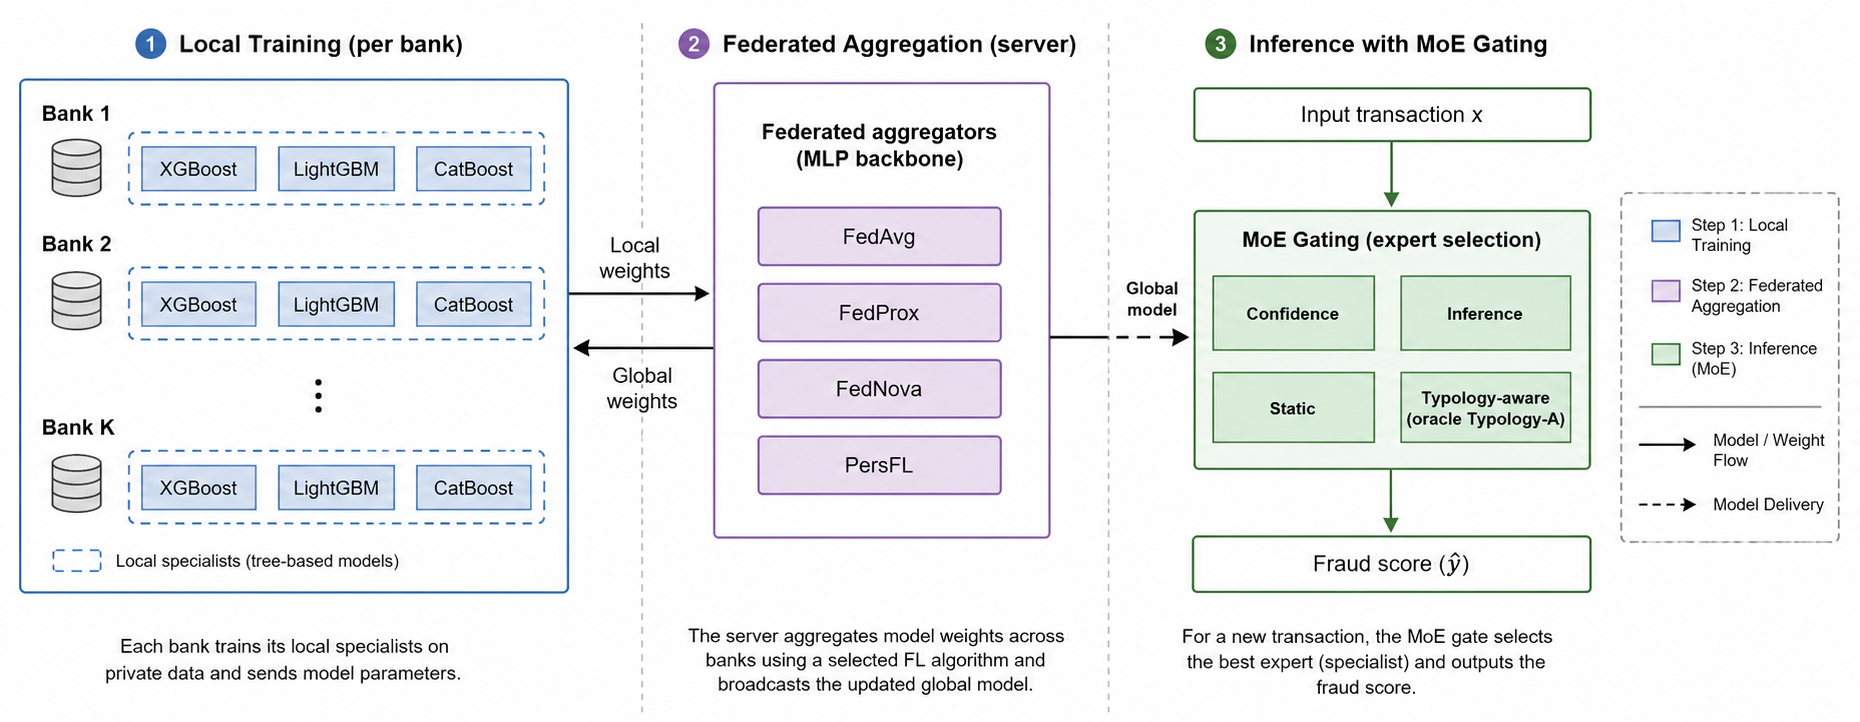
\includegraphics[width=\columnwidth]{fig1.png}
\caption{Three-phase expert-fusion pipeline: per-bank tree specialists, federated
MLP backbone aggregation across four banks, and a fusion gate at inference
(Static, Performance, Confidence, or oracle Typology-Aware$\dagger$). Each bank's
gate fuses its own three trees with the four shared backbones; no tree crosses a
bank boundary.}
\label{fig:arch}
\end{figure}

%%%%%%%%%%%%%%%%%%%%%%%%%%%%%%%%%%%%%%%%%%%%%%%%%%%%%%%%%%%%%%%%%%%%%%%%%%%%%%%%
\section{Introduction}

\subsection{Background}
Money laundering runs on fragmentation. Worth an estimated US\$2 to 3.1 trillion
a year \cite{r1}, the typologies that hide it (layering, smurfing, mule
networks) deliberately split funds across 4 to 7 banks \cite{r2}, \cite{r3}, so
one bank sees one slice and single-institution monitoring catches roughly 5\%.
No bank holds enough of any one typology to train a detector that generalises.
The direct fix, pooling the data, is illegal: GDPR, the Australian Privacy
Principles, APRA Prudential Standard CPS 234 \cite{r4} and competitive
sensitivity all rule it out. The question therefore shifts from ``can we share
data?'' to ``can we share models?''. That is the regime McMahan et al. \cite{r5}
built federated learning (FL) for: clients trade model weights, never raw
records.

FL does not eliminate the difficulty; three pressures stack. First, imbalance:
fraud prevalence runs from 0.10\% (SAML-D, IBM HI-Small) to 0.172\% (ULB), low
enough that AUROC saturates and AUPRC becomes the only metric worth reading.
Second, the non-IID split: banks specialise, so each client sees its own mix of
typologies, producing client drift \cite{r6}, \cite{r7}. Third, fraud labels in
SAML-D span 17 to 28 typologies \cite{r2}, so any global model is secretly a
mixture model. At extreme non-IID the three compound and the global model can
cave in.

\subsection{Related Work}
We screened 510 papers under PRISMA 2020 \cite{r8} and kept 42 with end-to-end
FL or MoE results on financial data. They fall into three groups, each leaving a
gap this paper addresses.

The first covers aggregation rules. FedAvg \cite{r5} computes a data-weighted
average and remains the default baseline, reported to degrade sharply under
non-IID; FedProx \cite{r9} adds a proximal term; FedNova \cite{r10} normalises
for unequal local step counts. Our sweep tests how much of that reported
fragility survives a multi-seed protocol.

The second personalises. PersFL/Per-FedAvg \cite{r11} keeps client-specific
weights alongside shared ones; Ditto \cite{r12} splits the two components. The
Dirichlet partition of Hsu et al. \cite{r13} is the standard non-IID simulator,
and we adopt it. In our grid PersFL is the only algorithm that never records
F1 = 0, at the price of a single unified global model.

The third combines experts. Adaptive mixtures \cite{r14} and sparsely gated MoE
\cite{r15} were extended by expert-choice routing \cite{r16}; federated variants
followed, with FedMix \cite{r31}, Marfoq et al. modelling each client as a
mixture of shared distributions \cite{r32}, and FedJETs routing to specialist
subsets \cite{r33}. pFL-Bench \cite{r34} gives personalisation the multi-seed
benchmark treatment we attempt for fraud. Our fusion layer is deliberately
simpler than these learned routers: per-bank scalar weights set on validation
folds, no input-conditional routing, hence ``expert fusion''. The strongest
standalone tabular models remain gradient-boosted trees (XGBoost \cite{r17},
LightGBM \cite{r18}, CatBoost \cite{r19}), our local experts; federated boosting
\cite{r35} targets vertical partitions, and direct FL-for-card-fraud work
\cite{r36} is single-dataset, single-seed. A separate selective-prediction
literature, from Chow's rejection rule \cite{r29} to conformal prediction
\cite{r30}, asks when a classifier should defer to a human; fraud work rarely
connects it to FL.

Similar limitations recur across all three groups: single seeds that hide
non-IID variance, single datasets, AUPRC-only reporting, and oracle gates mixed
in with deployable ones. To our knowledge no prior work evaluates multiple fraud
datasets, FL methods, fusion strategies, seeds, cost-aware metrics and a
deferral policy in one framework.

\subsection{Research Questions and Contributions}
Five research questions follow. RQ1: how does each FL algorithm degrade as the
Dirichlet concentration $\alpha$ falls from 0.50 to 0.05? RQ2: can an
expert-fusion layer bridge the divide between federated and centralised
learning? RQ3: which aggregation rule should a practitioner pick for a given
non-IID regime? RQ4: what is the utility cost of gradient noise and
sparsification? RQ5: can a cost-aware triage layer convert performance rankings
into an operational decision policy?

The contribution is a benchmark and a decision protocol rather than a new
learning algorithm. First, a matched-protocol non-IID benchmark: eleven
strategies (four FL algorithms, three tree experts, four fusion gates) $\times$
three dataset families $\times$ three $\alpha$ settings $\times$ five seeds
gives 495 main-sweep runs, and a 60-round ULB noise-robustness grid brings the
total to 516, with every partition seed derived only from (seed, dataset,
$\alpha$). Second, a two-convention statistical reading of the fusion layer: the
gates beat the FL family mean on all three datasets and hold the best overall
Friedman rank, yet never beat the per-cell best backbone, and their weights sit
close to uniform, so the layer is a weighted ensemble rather than a router.
Third, an algorithm-survival map indexed by non-IID regime and reported as seed
frequencies rather than verdicts. Fourth, a triage layer (per-bank conformal
thresholds, a Chow-style defer band, a capacity cap) that auto-clears 74 to
99.8\% of transactions at recall 80 with a 4 to 5\% defer rate.

%%%%%%%%%%%%%%%%%%%%%%%%%%%%%%%%%%%%%%%%%%%%%%%%%%%%%%%%%%%%%%%%%%%%%%%%%%%%%%%%
\section{Methods}

\subsection{System Overview}
The pipeline has three phases (Fig.~\ref{fig:arch}). Phase 1 trains each bank's
specialist classifiers on its private slice. Phase 2 federates a shared MLP
backbone across banks. At inference, Phase 3 sends each transaction through a
fusion gate blending local specialists with the federated backbones. Phase 2
reuses Phase 1's partition, and the Phase 3 gates are tuned on the per-bank
validation folds the earlier phases leave behind. Seven experts sit under each
bank's gate: the four shared FL-MLP backbones (PersFL contributes that bank's
personalised copy) and the bank's own three trees, which never leave it.

\subsection{Data Pipeline}
Three public benchmark families stress-test the pipeline across scales and
feature regimes. ULB Credit Card \cite{r20} contains 284,807 transactions at
0.172\% fraud with 29 PCA features. SAML-D \cite{r2} is larger: 9.5 million
transactions at 0.10\% fraud, with 10 engineered features carrying typological
structure. IBM AML \cite{r21} is used at HI-Small scale, roughly 5.1 million
transactions at 0.10\% fraud, whose held-out window contains 761,753
transactions with 1,561 frauds (0.21\%). Every dataset passes through a log1p
transform on Amount and removal of the raw Time column, with StandardScaler
fitted on each bank's training fold only.

Federated partitioning simulates $N = 4$ banks by drawing fraud indices from a
Dirichlet prior and distributing legitimate indices uniformly. Given the
positive index set $I^{+}$ and concentration $\alpha$:

\begin{equation}
p \sim \mathrm{Dir}(\alpha \cdot \mathbf{1}_{N}), \quad n_i^{+} = p_i \cdot |I^{+}|, \quad n_i^{-} = |I^{-}|/N
\end{equation}

The $\alpha$ sweep covers \{0.05, 0.10, 0.50\}. The partition RNG is seeded by a
hash of (seed, dataset, $\alpha$) alone, so any cell reproduces by itself.
Per-bank splits are temporal 70/15/15. Class imbalance is handled with per-bank
SMOTE \cite{r22} at k\_neighbors = min(3, n\_fraud $-$ 1); for all tree models
scale\_pos\_weight is n\_neg/n\_pos.

\subsection{Phase 1: Per-Bank Local Specialists}
Each bank trains three gradient-boosted classifiers locally: XGBoost
(n\_estimators = 200, max\_depth = 6, eval\_metric = aucpr) \cite{r17}, LightGBM
(n\_estimators = 200, max\_depth = 6) \cite{r18} and CatBoost (iterations = 200,
depth = 6, eval\_metric = PRAUC) \cite{r19}. Tree ensembles remain dominant for
tabular fraud, and each bank's local distribution stays well-conditioned
whatever happens elsewhere in the federation.

\subsection{Phase 2: Federated MLP Aggregation}
The backbone is a scikit-learn MLPClassifier with hidden layers (128, 64, 32),
ReLU activations, Adam (lr = 10\textsuperscript{$-$3}), batch size 128 and
log-loss, trained for 20 rounds. Each round every bank continues from the
current global weights, so an initialised network is never reinitialised. FedAvg
\cite{r5} aggregates client weights by sample count (2). FedProx \cite{r9} adds
a proximal regulariser at $\mu$ = 0.01 (3); sklearn exposes no per-step loss
hook, so the term is applied per epoch as a documented pull
$\min(\eta \mu S, 0.5)$ toward the global weights ($S$ = steps per epoch).
FedNova \cite{r10} normalises each client's update by its local step count
$\tau_i = 5 \lceil n_i/128 \rceil$ before aggregation (4). PersFL \cite{r11}
blends bank $i$'s weights 50/50 with the global model after each local fit, and
those personalised copies are what Phase 3 evaluates.

\begin{equation}
w^{(t+1)} = \textstyle\sum_{i} \, (n_i / N_{\mathrm{tot}}) \cdot w_i^{(t)}
\end{equation}
\begin{equation}
L_i(w) = \mathrm{BCE}(w; D_i) + (\mu/2) \, \lVert w - w^{(t)} \rVert^{2}, \quad \mu = 0.01
\end{equation}
\begin{equation}
w^{(t+1)} = w^{(t)} + \tau_{\mathrm{eff}} \textstyle\sum_i \bigl[ n_i \tau_i \big/ \sum_j n_j \tau_j \bigr] d_i
\end{equation}

\subsection{Phase 3: Expert-Fusion Gating}
Write $p_e(x)$ for expert $e$'s probability on transaction $x$. Each bank's gate
fuses its seven experts as $\hat{y}(x) = \sum_e g_e \cdot p_e(x)$, and the four
variants differ only in how they set $g_e$. The weights are per-bank scalars
computed once on the validation fold; nothing is input-conditional and no router
is learned. Static is the baseline, $g_e = 1/E$. Performance weights by
validation F2, $g_e = \mathrm{F2}_e^{\mathrm{val}} / \sum_{e'}
\mathrm{F2}_{e'}^{\mathrm{val}}$. Confidence rewards experts whose scores sit far
from the decision boundary, defined in (5), and never looks at a label.
Typology-Aware$\dagger$ routes on the ground-truth fraud type $t$,
$g_e(x|t) = \mathrm{F1}_e^{\mathrm{val}}(t) / \sum_{e'}
\mathrm{F1}_{e'}^{\mathrm{val}}(t)$, which is why it cannot ship: the label is
absent at inference, so we carry it as an upper bound only, tagged $\dagger$
wherever it appears.

\begin{equation}
g_e = c_e \big/ \textstyle\sum_{e'} c_{e'}, \quad c_e = \mathrm{E}_x \bigl[ \, | p_e(x) - 0.5 | \times 2 \, \bigr]
\end{equation}

\subsection{Gradient-Noise and Sparsification Robustness}
This ablation predates the canonical sweep and runs on a separate 60-round ULB
implementation with a four-layer PyTorch backbone, five banks and
$\alpha$ = 0.5. Two mechanisms are measured, both as robustness experiments.
\emph{Gaussian gradient noise}: gradients are clipped each step to norm
$C$ = 1.0, then noise is added with $\sigma = zC/n_b$ at $z$ = 1.1, the
mechanism (though not the accounting) of DP-SGD \cite{r23}, \cite{r24}. There is
no privacy accountant and no differential-privacy claim; an $\varepsilon$ of 4.0
quoted in earlier drafts is withdrawn. \emph{Top-K sparsification} \cite{r25}:
only the top 1\% of gradient entries by magnitude are transmitted each round,
cutting communication by roughly two orders of magnitude.

\subsection{Evaluation Protocol}
AUPRC is the primary metric, since AUROC turns overly optimistic when the
positive class sits near 0.1 to 0.2\%. Secondary metrics are final-round F1 at
the actual operating point rather than the best across rounds, F2, Matthews
correlation coefficient, and per-bank worst-case F1. All main results are 5-seed
mean $\pm$ std.

For statistical testing we use a Friedman $\chi^2$ test over the 45
seed-condition blocks \cite{r28}, followed by Wilcoxon signed-rank tests under
two conventions, family means (does a gate beat the average backbone?) and
per-cell bests (does the best gate beat the best backbone?), with Cliff's delta
effect sizes \cite{r27}. With five seeds a per-$\alpha$ two-sided Wilcoxon
cannot go below p = 0.0625, so the pooled 15-block tests carry the p-values,
with a resolution floor of p = 6.1$\times$10\textsuperscript{$-$5} at roughly 40
single-GPU hours. Tables report raw p-values; every significance call survives a
Holm--Bonferroni adjustment within its comparison family. A cost-aware layer
varies the relative cost of false negatives: expected loss is
$L(\rho) = \mathrm{FN} \cdot \rho + \mathrm{FP}$, across
$\rho \in \{10, \ldots, 5000\}$. On hyperparameters our policy is symmetry over
search: both expert families run library-typical settings at matched budgets
with no per-dataset tuning.

\subsection{Reproducibility}
All experiments ran across five seeds (42, 0, 1, 2, 3) on single NVIDIA Tesla
P100 16 GB GPUs on Kaggle's standard image (Python 3.12). Because the partition
seed depends only on (seed, dataset, $\alpha$), the grid splits across sessions
and machines onto identical cells; the repository contains the sweep scripts,
the triage package and complete per-cell outputs. Two forensic findings shaped
this section: a reinitialising FL loop, whose byte-identical rows fabricated the
retracted 0.699 ULB plateau and the FedProx tenfold claim, and RNG tracing that
showed our earliest result set came from unmerged code. The PyTorch privacy grid
keeps one caveat: its global seed was not fixed, so its numbers carry
floating-point-level noise. Table \ref{tab:hyper} lists the hyperparameters.

\begin{table}[!tb]
\caption{Consolidated Hyperparameters (s = sweep, g = privacy grid)}\label{tab:hyper}
\centering\scriptsize
\setlength{\tabcolsep}{3pt}
\begin{tabular}{@{}ll|ll@{}}
\hline
\textbf{Param} & \textbf{Value} & \textbf{Param} & \textbf{Value} \\ \hline
Banks $N$ & 4 s / 5 g & n\_est. / depth & 200 / 6 s \\
Rounds$\times$epochs & 20$\times$5 s / 60$\times$3 g & SMOTE $k$ & min(3, $n_{\mathrm{fraud}}{-}1$) \\
MLP hidden & (128, 64, 32) s & Noise $C$, $z$ & 1.0, 1.1 g \\
Partition seed & hash(seed, data, $\alpha$) & Top-K & 0.01 g \\
PersFL blend & 0.5 local / 0.5 global & Recall target & 0.80 \\
FedNova $\tau_i$ & $5\lceil n_i/128 \rceil$ s & Defer cap & 5\% \\
Batch / LR & 128 / $1{\times}10^{-3}$ & FedProx $\mu$ & 0.01 \\
Dirichlet $\alpha$ & \{.05, .10, .50\} s / 0.4 g & Seeds & \{42, 0, 1, 2, 3\} \\ \hline
\end{tabular}
\end{table}

%%%%%%%%%%%%%%%%%%%%%%%%%%%%%%%%%%%%%%%%%%%%%%%%%%%%%%%%%%%%%%%%%%%%%%%%%%%%%%%%
\section{Experiments and Results}

Eleven strategies, three dataset families, three Dirichlet settings and five
seeds give 495 main-sweep runs, plus 21 populated cells of a 60-round ULB
noise-robustness grid, 516 in total. Every headline below is a 5-seed mean
$\pm$ std unless stated otherwise.

\subsection{Heterogeneity Sweep (RQ1)}
Take AUPRC for the eleven strategies' seed means on a dataset and correlate with
$\alpha$. On ULB that correlation is strong and positive: Spearman $\rho$ =
+0.943, p = 2$\times$10\textsuperscript{$-$16}, n = 33. The fall-off is gentle
(FedAvg means 0.609 at $\alpha$ = 0.50, 0.425 at 0.10, 0.318 at 0.05), and
Fig.~\ref{fig:sweep} shows it holding for every backbone and gate, the oracle
included.

The AML datasets behave differently, and differently from each other. On SAML-D,
$\rho$ = +0.772 (p = 1.5$\times$10\textsuperscript{$-$7}), but the mean hides the
mechanism: at $\alpha$ = 0.05 four of five seeds send every standard backbone to
AUPRC 0.002 to 0.004 together, while the fifth leaves them all intact around
0.09. Survival at extreme skew is decided by the partition draw; FedAvg and
FedProx sit within a hair of each other in every cell. On IBM HI-Small the
correlation disappears altogether ($\rho$ = +0.150, p = 0.40): performance is
nearly flat in $\alpha$ (FedAvg 0.033 / 0.027 / 0.039), so what limits IBM is
feature signal. Non-IID degradation is thus three curves: graceful on PCA
features, a partition-induced instability on SAML-D, mostly absent on IBM.

\begin{figure}[!tb]
\centering
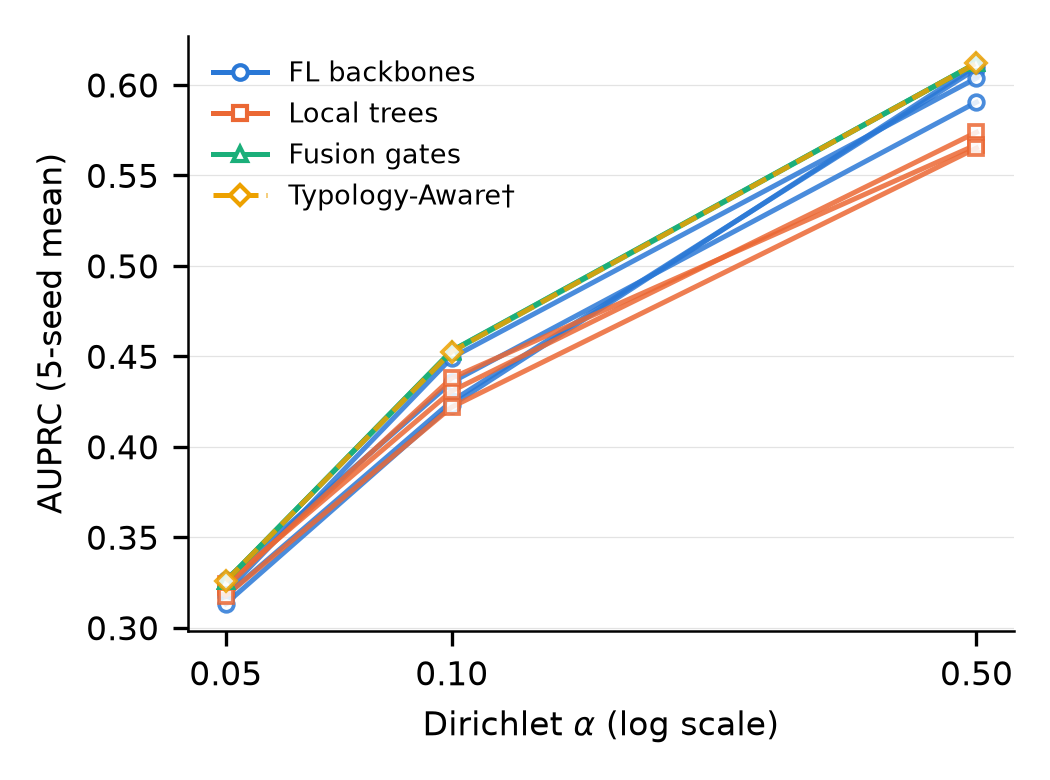
\includegraphics[width=0.70\columnwidth]{fig2.png}
\caption{ULB AUPRC vs Dirichlet $\alpha$, 5-seed means, coloured by family.
Degradation is monotonic ($\rho$ = +0.943) and family ordering is stable.}
\label{fig:sweep}
\end{figure}

\subsection{Expert Fusion Under Two Conventions (RQ2)}
Table \ref{tab:cross} is the $\alpha$ = 0.5 cross-dataset cell. On ULB the gates
(0.612 $\pm$ 0.151) top the deployable table, a nose above the best backbone
(FedNova 0.611) and clearly above the trees (0.565 to 0.574). On SAML-D and IBM
HI-Small the trees lead (0.079, 0.051) with the gates just behind, well clear of
FL. The oracle escapes the pack only on the AML datasets (0.051 IBM, 0.083
SAML-D), bounding what a better typology detector could add. On ULB it cannot
escape by construction: with one fraud typology its weights fall back to the
performance gate's for 99.8\% of transactions, so the routing headroom is
exactly zero.

\begin{table}[!tb]
\caption{$\alpha$ = 0.5 Cross-Dataset AUPRC, 5-Seed Mean $\pm$ Std}\label{tab:cross}
\centering\scriptsize
\setlength{\tabcolsep}{4pt}
\begin{tabular}{@{}lccc@{}}
\hline
\textbf{Strategy} & \textbf{ULB} & \textbf{IBM HI-S} & \textbf{SAML-D} \\ \hline
FedAvg & 0.609$\pm$0.151 & 0.039$\pm$0.005 & 0.075$\pm$0.027 \\
FedProx & 0.604$\pm$0.148 & 0.037$\pm$0.009 & 0.070$\pm$0.026 \\
FedNova & 0.611$\pm$0.151 & 0.043$\pm$0.006 & 0.071$\pm$0.026 \\
PersFL & 0.590$\pm$0.122 & 0.033$\pm$0.008 & 0.073$\pm$0.021 \\
XGBoost & 0.574$\pm$0.151 & 0.043$\pm$0.002 & 0.080$\pm$0.013 \\
LightGBM & 0.567$\pm$0.153 & 0.051$\pm$0.001 & 0.079$\pm$0.013 \\
CatBoost & 0.565$\pm$0.157 & 0.044$\pm$0.002 & 0.077$\pm$0.007 \\
Fusion-Static & 0.612$\pm$0.151 & 0.044$\pm$0.003 & 0.076$\pm$0.027 \\
Fusion-Perf & 0.612$\pm$0.151 & 0.044$\pm$0.003 & 0.077$\pm$0.027 \\
Fusion-Conf & 0.612$\pm$0.151 & 0.044$\pm$0.003 & 0.076$\pm$0.027 \\
Fusion-TypAw$\dagger$ & 0.612$\pm$0.151 & 0.051$\pm$0.005 & 0.083$\pm$0.020 \\ \hline
\end{tabular}
\par\smallskip\raggedright\scriptsize $\dagger$ Oracle gate; upper bound only, never deployed.
\end{table}

Whether the gate ``wins'' depends on the question, so Table \ref{tab:conv} asks
both. Against the FL \emph{family mean} the gates win on every dataset (pooled
15-block Wilcoxon p = 0.030 / 6$\times$10\textsuperscript{$-$5} / 0.012);
against the \emph{per-cell best} backbone they are a coin flip everywhere
(p $\ge$ 0.76). Both are true at once: the gate is a hedge. Practitioners cannot
know in advance which backbone a partition will favour, and the near-uniform
blend lands at or above the field's centre of mass. The measured weights agree:
the top expert's mean weight stays between 0.143 (uniform for seven experts) and
0.29, and the nominal top expert flips with the seed. As an ablation of the
weighting function the verdict is that it barely matters: static, F2-weighted
and confidence weighting land within 0.001 AUPRC of one another everywhere. The
reason is mechanical. Linearly normalising validation scores that all sit in a
narrow band gives near-uniform weights by construction, and on 99.8\%-negative
data the confidence signal mostly records sigmoid saturation. Expert rankings
also correlate at 0.37 to 0.93, and AUPRC is rank-based, so perturbations this
small have nothing to move. Nor is this an implementation artefact: replayed on
the captured probabilities, sharpened weights change nothing and rank-normalising
before blending \emph{costs} 0.015 AUPRC on ULB and SAML-D.

\begin{table}[!tb]
\caption{Deployable Fusion Gates vs Other Families, Pooled 15-Block Wilcoxon (p / Cliff's $\delta$)}\label{tab:conv}
\centering\scriptsize
\setlength{\tabcolsep}{4pt}
\begin{tabular}{@{}lccc@{}}
\hline
\textbf{Comparison} & \textbf{ULB} & \textbf{IBM HI-S} & \textbf{SAML-D} \\ \hline
vs FL, family mean & \textbf{.030} / +.10 & \textbf{6e-5} / +.54 & \textbf{.012} / +.17 \\
vs FL, per-cell best & .80 / $-$.00 & .76 / +.12 & .85 / +.04 \\
vs trees, family mean & \textbf{1.2e-4} / +.18 & .083 / $-$.56 & .055 / $-$.23 \\
vs trees, per-cell best & \textbf{.002} / +.16 & \textbf{.011} / $-$.72 & \textbf{.018} / $-$.25 \\ \hline
\end{tabular}
\par\smallskip\raggedright\scriptsize Bold: p $<$ 0.05, all surviving Holm--Bonferroni. Positive $\delta$ favours the gates; on IBM and SAML-D the best-vs-best results favour the \emph{trees}.
\end{table}

Against the centralised pooled baseline the ceiling holds everywhere: XGBoost
reaches 0.764 on ULB, CatBoost 0.071 on IBM and 0.089 on SAML-D, leaving the
best deployable method (Fusion-Static 0.612, Fusion-Perf 0.044 and 0.077) 0.152,
0.027 and 0.012 short. These baselines are single pooled runs on a fixed
temporal split; XGBoost was byte-identical across three sessions and CatBoost
moved by $\le$0.001, while centralised LightGBM is degenerate and excluded
pending a fix. One earlier draft had a seed-42 cell beating the baseline by
+0.089; the audited pipeline puts that cell 0.181 \emph{below} it. Over all 45
blocks the Friedman test ranks the deployable families gates 4.99, trees 5.61,
FL 7.77 ($\chi^2$ = 110.2, p = 5$\times$10\textsuperscript{$-$19}; the oracle
sits at 3.11), and Fusion-Perf is the best single deployable strategy at mean
rank 4.48. RQ2 therefore gets a two-part answer: fusion is the best deployable
family on average, and the gap to pooled raw data does not close.

\begin{figure}[!tb]
\centering
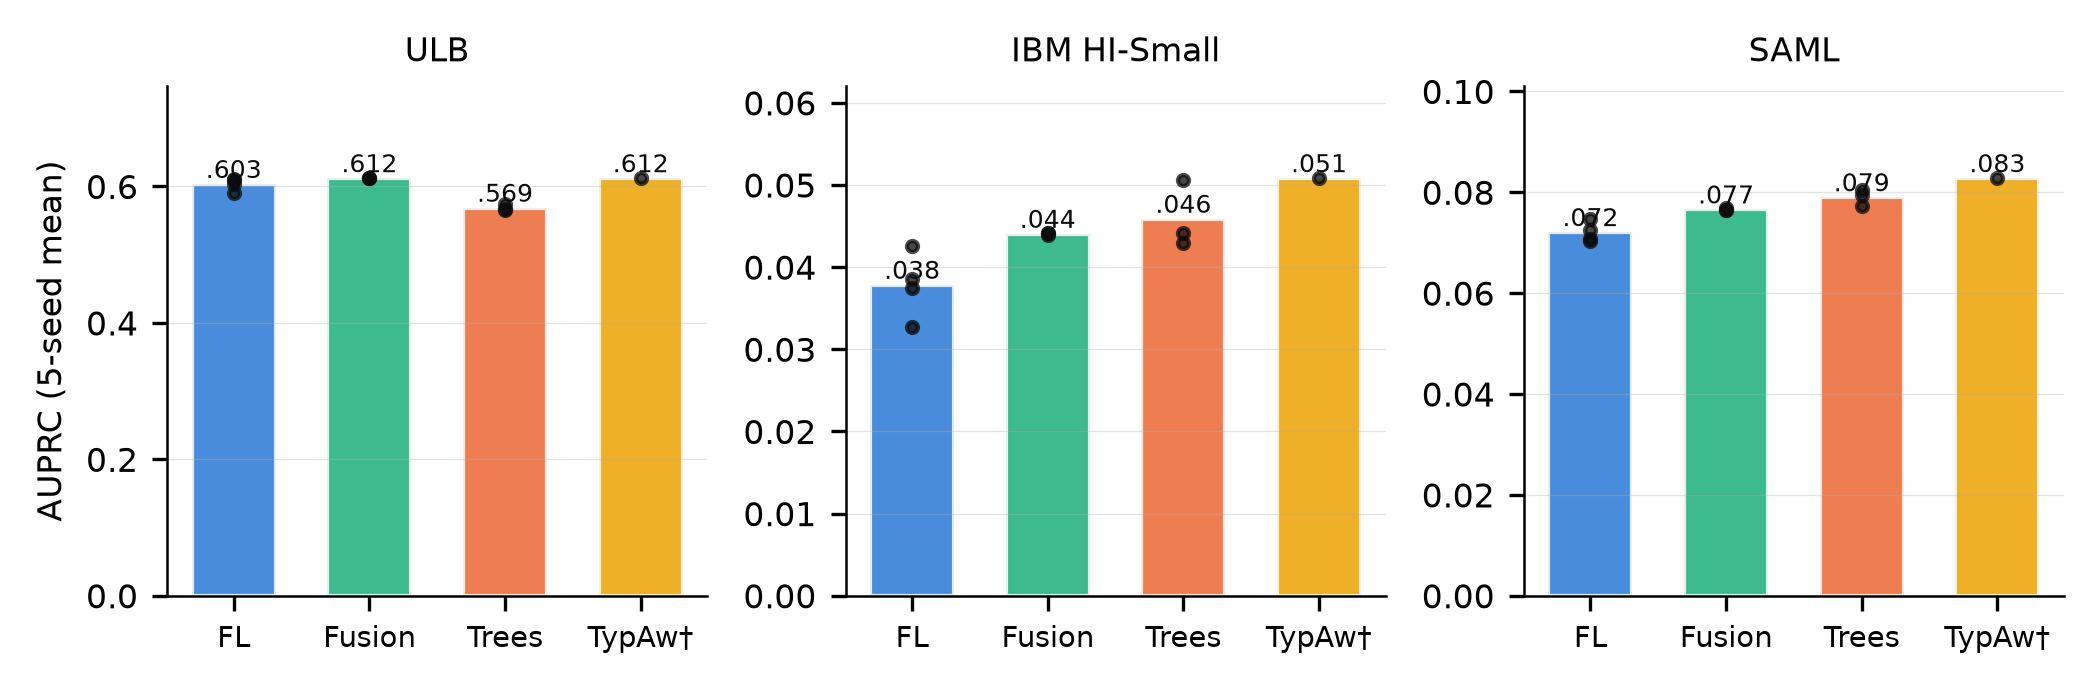
\includegraphics[width=0.86\columnwidth]{fig3.png}
\caption{Family-level AUPRC at $\alpha$ = 0.5; bars are family means, dots
individual strategies. Note the per-panel scales.}
\label{fig:family}
\end{figure}

\subsection{FL Algorithm Survival (RQ3)}
Table \ref{tab:survival} counts, for each backbone, the seeds whose final F1
lands at exactly zero, turning operating-point collapse into a frequency. Three
patterns emerge that the deterministic verdicts of earlier drafts had flattened.
First, collapse at $\alpha$ = 0.05 is a partition-dependent variability, and a
largely strategy-blind one: on SAML-D, seeds 0, 1, 3 and 42 take every standard
backbone down together while seed 2 spares them all, and on IBM exactly one seed
zeroes FedAvg, FedProx and FedNova at once. Second, FedNova owns the most
fragile operating point: no other backbone hits F1 = 0 in four of five SAML-D
seeds at $\alpha$ = 0.05, and at $\alpha$ = 0.10 it is the only backbone to
record a zero at all. Third, PersFL never records F1 = 0 anywhere, posting 2 to
10$\times$ the AUPRC of the other backbones inside collapsed partitions, though
two SAML-D seeds still leave its AUPRC under 0.005.

Cost re-ranking sharpens the deployment picture. Across the 81
(dataset, $\alpha$, $\rho$) cells, the method with the best AUPRC is also the
cost-best deployable method in only 10; the gates take 45 cells, concentrated at
$\rho \le$ 50 (17 of 27), and PersFL takes 23, concentrated at $\rho \ge$ 1000
(15 of 27). Review-cheap regimes favour a gate, miss-expensive regimes favour
personalisation.

\begin{table}[!tb]
\caption{Operating-Point Collapse Frequency: Seeds (of 5) with F1 = 0. U/S/I = ULB/SAML-D/IBM HI-Small}\label{tab:survival}
\centering\scriptsize
\setlength{\tabcolsep}{4.2pt}
\begin{tabular}{@{}lccccccccc@{}}
\hline
\textbf{Algo} & \textbf{U.5} & \textbf{U.1} & \textbf{U.05} & \textbf{S.5} & \textbf{S.1} & \textbf{S.05} & \textbf{I.5} & \textbf{I.1} & \textbf{I.05} \\ \hline
FedAvg & 0 & 0 & 0 & 0 & 0 & 1 & 0 & 0 & 1 \\
FedProx & 0 & 0 & 0 & 0 & 0 & 1 & 0 & 0 & 1 \\
FedNova & 0 & 0 & 0 & 0 & 1 & 4 & 0 & 0 & 1 \\
PersFL & 0 & 0 & 0 & 0 & 0 & 0 & 0 & 0 & 0 \\ \hline
\end{tabular}
\end{table}

\subsection{Gradient-Noise and Sparsification Robustness (RQ4)}
Table \ref{tab:privacy} reports final-round AUC from the 60-round ULB grid. This
grid predates the canonical sweep (PyTorch, single seed), so we read it for
deltas rather than absolute levels. The noise result is the most notable:
relative to clean runs, final-round AUC shifts by at most 0.012 on the MLP and
0.003 on logistic regression, slightly upward if anything and inside
seed-to-seed variance, so for rank-ordering the noise is essentially free.
Sparsification costs 0.02 to 0.05 AUC on the MLP and around 0.005 on LR. The
worst case is FedNova with sparsification, which reaches a final F1 of only
0.009 and is unusable regardless of the AUC curve. At the top end the MLP
reaches 0.984 AUC (FedNova with noise) against 0.957 for LR; closing that gap
costs 10 to 25 times more compute per round, so when communication is the
constraint LR with sparsification is reasonable.

These are robustness numbers; privacy is not claimed. There is no R\'enyi-DP
accountant, no subsampling amplification argument and no auditable $\varepsilon$
at the end of training, so Table \ref{tab:privacy} labels the mechanism Gaussian
noise. Turning these figures into a guarantee needs an accountant.

\begin{table}[!tb]
\caption{ULB 60-Round Final-Round AUC Under Gradient Noise (Single Seed, Seed 42)}\label{tab:privacy}
\centering\scriptsize
\setlength{\tabcolsep}{4.2pt}
\begin{tabular}{@{}lcccccc@{}}
\hline
\textbf{FL algo} & \textbf{\shortstack{MLP\\Clean}} & \textbf{\shortstack{MLP\\Noise}} & \textbf{\shortstack{MLP\\Spars}} & \textbf{\shortstack{LR\\Clean}} & \textbf{\shortstack{LR\\Noise}} & \textbf{\shortstack{LR\\Spars}} \\ \hline
FedAvg & 0.966 & 0.973 & 0.945 & 0.960 & 0.958 & 0.955 \\
FedProx & 0.974 & 0.977 & 0.957 & 0.960 & 0.963 & 0.957 \\
FedNova & 0.980 & 0.984 & 0.960 & n/a & n/a & n/a \\
PersFL & 0.962 & 0.974 & 0.948 & 0.960 & 0.962 & 0.962 \\ \hline
\end{tabular}
\end{table}

\subsection{From Rankings to Decisions: the Triage Layer (RQ5)}
The two-convention result leaves a practical question: if no deployable strategy
reliably beats the field, what should a fraud team run? Our answer optimises the
decision instead of the ranking. The triage layer applies, per bank, a
split-conformal clear threshold at a recall-80 target (with a plain-threshold
fallback where calibration frauds are too few), a Chow-style defer band
\cite{r29} whose width follows $\rho = c_{\mathrm{FN}}/c_{\mathrm{FP}}$, and a
5\% review-capacity cap. Everything below the band auto-clears, the band defers
to human review, and the rest alerts.

Table \ref{tab:triage} pools 3 $\alpha$ $\times$ 5 seeds $\times$ 6 $\rho$ per
dataset. Three properties matter. First, the auto-clear rate is the dataset's
difficulty made visible: 99.8\% of ULB transactions clear at recall 80, 89\% on
IBM, 74\% on SAML-D. Second, the defer rate barely moves (3.8 to 4.6\%): the
capacity cap binds. Third, expected cost per transaction moves by only 0.9 to
3.6\% while $\rho$ sweeps from 1 to 50, so a team that cannot pin its cost ratio
within a factor of fifty still lands on the same policy. Conformal validity
holds for 64 to 79\% of bank-cells, the rest falling back to threshold mode; the
soft spot is ULB $\alpha$ = 0.5, where the test window holds only 52 frauds.

\begin{table}[!tb]
\caption{Triage Layer at Recall-80, Pooled over $\alpha$, Seeds and $\rho$}\label{tab:triage}
\centering\scriptsize
\setlength{\tabcolsep}{4pt}
\begin{tabular}{@{}lccc@{}}
\hline
 & \textbf{ULB} & \textbf{IBM HI-S} & \textbf{SAML-D} \\ \hline
Auto-clear rate & 0.998 & 0.894 & 0.735 \\
Defer rate & 0.038 & 0.045 & 0.046 \\
Policy miss rate & 0.081 & 0.050 & 0.074 \\
Conformal coverage valid & 0.64 & 0.79 & 0.75 \\
Cost drift, $\rho$: 1$\to$50 & +3.6\% & +1.5\% & +0.9\% \\ \hline
\end{tabular}
\end{table}

\subsection{Per-Bank Fairness}
Across every populated ULB noise-grid cell, Jain's index sits at 0.9999 or
better and $\sigma$-AUC stays under 0.02, so the aggregation itself treats banks
evenly. The sweep-level picture is harsher: at $\alpha \le$ 0.10, at least one
bank posts a worst-case F1 of zero in 110/110 ULB cells, 104/110 SAML-D cells
and 83/110 IBM cells (36, 19 and 3 of 55 at $\alpha$ = 0.5). These zeroes are a
property of the data allocation, and they make the strongest case we know for
per-bank triage thresholds.

%%%%%%%%%%%%%%%%%%%%%%%%%%%%%%%%%%%%%%%%%%%%%%%%%%%%%%%%%%%%%%%%%%%%%%%%%%%%%%%%
\section{Discussion}

\subsection{Principal Findings}
RQ1's answer is that no single degradation curve exists; the shape belongs to
the dataset. On ULB all eleven strategies decline smoothly in lockstep as
$\alpha$ falls; on SAML-D the decline is stochastic, driven by the partition
draw; on IBM HI-Small heterogeneity barely registers. Verifying partition
structure therefore matters more than choosing among FedAvg-family aggregators.

The fusion result must be read under two conventions: the best deployable
Friedman rank exceeds the FL family mean in every cell, yet never the per-cell
best backbone, whose identity shifts with the seed. The gates are weighted
ensembles whose value is hedging against the unanswerable question of which
backbone a given quarter's data will favour. PersFL, meanwhile, buys a
performance floor at the cost of the single global model that is FL's principal
communication advantage.

The cost and triage results prove the most broadly applicable. Best-AUPRC and
cost-best coincide in only 10 of 81 cells, so a leaderboard alone misallocates
review budget in the other 71. None of this depended on a superior model, only a
better decision rule.

\subsection{Limitations}
(1) The noise ablation is a robustness experiment; no differential-privacy
guarantee is claimed anywhere in this paper, and the grid is single-seed and
predates the canonical pipeline. (2) The Typology-Aware gate uses ground-truth
fraud-type labels at inference and is an upper bound only. (3) The centralised
baselines are single pooled runs, and the centralised LightGBM path is
degenerate and excluded pending a fix. (4) Five seeds keeps every per-$\alpha$
Wilcoxon at or above p = 0.0625 by construction; the pooled tests carry the
inference, and per-cell standard deviations remain wide. (5) Conformal validity
holds for 64 to 79\% of bank-cells, with ULB $\alpha$ = 0.5 the weakest slice.
(6) At $\alpha$ = 0.05 the Dirichlet sampler legitimately allocates zero fraud
cases to some banks, flooring per-bank evaluation. (7) The banks are simulated
silos and the heterogeneity is label-prevalence skew, whereas real silos also
differ in features and schemas, so ``cross-bank'' and ``deployable'' are
within-simulation claims and a pilot on real institutions remains future work.

\subsection{Comparison with Prior Work}
Across the 42 papers retained under the PRISMA protocol \cite{r8}, most report
AUPRC on a single dataset with a single seed against one or two FL baselines;
oracle and deployable gating are rarely distinguished, and asymmetric loss
rarely considered. This benchmark expands along all of those dimensions, and its
two-convention reporting separates ``beats the average'' from ``beats the
best''.

%%%%%%%%%%%%%%%%%%%%%%%%%%%%%%%%%%%%%%%%%%%%%%%%%%%%%%%%%%%%%%%%%%%%%%%%%%%%%%%%
\section{Conclusion and Future Work}

We asked whether FL with an expert-fusion layer on top is an efficient
architecture for cross-bank fraud detection. Four findings emerge. First, the
benchmark: 516 runs over three dataset families, eleven strategies, three
Dirichlet regimes and five seeds, with partitions reproducible cell by cell.
Second, a two-convention verdict on the gate: best deployable Friedman rank and
a win over the FL family mean on all three datasets, no win over the per-cell
best backbone, near-uniform weights; the gate is a computationally inexpensive
hedge against backbone selection. Third, a survival map rewritten as
frequencies: collapse at extreme skew is a partition-induced instability,
FedNova's operating point is the most fragile, and PersFL never hits F1 = 0.
Fourth, a triage layer that turns a flat ranking into a policy, auto-clearing 74
to 99.8\% of transactions at recall 80 with a 4 to 5\% defer rate.

Several directions follow from the limitations. The most immediate is adding a
real differential-privacy mechanism with an accountant so the gradient-noise
robustness numbers can become privacy numbers. Three extensions would deepen the
benchmark: a genuinely per-sample learned gate, the only variant that showed any
signal in our post-hoc probes; a federated gradient-boosting baseline to attack
the residual tree advantage on the AML datasets; and a canonical-protocol rerun
at IBM's larger scales. Finally, scaling past four banks and piloting under
Australian data-locality rules would test these findings at deployment scale.

%%%%%%%%%%%%%%%%%%%%%%%%%%%%%%%%%%%%%%%%%%%%%%%%%%%%%%%%%%%%%%%%%%%%%%%%%%%%%%%%
\section*{Acknowledgment}
The authors acknowledge the Faculty of Engineering and Information Technology,
University of Technology Sydney, and the providers of the public datasets used
in this study. Implementation and evaluation scripts:
\url{https://github.com/nordonezc/moe_fraud_detection}.

%%%%%%%%%%%%%%%%%%%%%%%%%%%%%%%%%%%%%%%%%%%%%%%%%%%%%%%%%%%%%%%%%%%%%%%%%%%%%%%%
\begin{thebibliography}{99}
\bibitem{r1} B. Unger and J. Ferwerda, \emph{Money Laundering in the Real Estate Sector}. Cheltenham, U.K.: Edward Elgar, 2011.
\bibitem{r2} B. Oztas et al., ``Enhancing anti-money laundering: Development of a synthetic transaction monitoring dataset (SAML-D),'' in \emph{Proc. IEEE ICEBE}, 2023, pp. 47--54.
\bibitem{r3} P. Reuter and E. M. Truman, \emph{Chasing Dirty Money: The Fight Against Money Laundering}. Washington, DC, USA: Peterson Inst. Int. Econ., 2004.
\bibitem{r4} Australian Prudential Regulation Authority, ``Prudential standard CPS 234: Information security,'' APRA, Sydney, Australia, 2019.
\bibitem{r5} H. B. McMahan et al., ``Communication-efficient learning of deep networks from decentralized data,'' in \emph{Proc. AISTATS}, vol. 54, 2017, pp. 1273--1282.
\bibitem{r6} Y. Zhao et al., ``Federated learning with non-IID data,'' 2018, arXiv:1806.00582.
\bibitem{r7} S. P. Karimireddy et al., ``SCAFFOLD: Stochastic controlled averaging for federated learning,'' in \emph{Proc. ICML}, vol. 119, 2020, pp. 5132--5143.
\bibitem{r8} M. J. Page et al., ``The PRISMA 2020 statement: An updated guideline for reporting systematic reviews,'' \emph{BMJ}, vol. 372, Art. no. n71, 2021.
\bibitem{r9} T. Li et al., ``Federated optimization in heterogeneous networks,'' in \emph{Proc. MLSys}, vol. 2, 2020, pp. 429--450.
\bibitem{r10} J. Wang et al., ``Tackling the objective inconsistency problem in heterogeneous federated optimization,'' in \emph{NeurIPS}, vol. 33, 2020, pp. 7611--7623.
\bibitem{r11} A. Fallah, A. Mokhtari, and A. Ozdaglar, ``Personalized federated learning with theoretical guarantees: A model-agnostic meta-learning approach,'' in \emph{NeurIPS}, vol. 33, 2020, pp. 3557--3568.
\bibitem{r12} T. Li et al., ``Ditto: Fair and robust federated learning through personalization,'' in \emph{Proc. ICML}, 2021, pp. 6357--6368.

\bibitem{r13} T.-M. H. Hsu, H. Qi, and M. Brown, ``Measuring the effects of non-identical data distribution for federated visual classification,'' 2019, arXiv:1909.06335.
\bibitem{r14} R. A. Jacobs, M. I. Jordan, S. J. Nowlan, and G. E. Hinton, ``Adaptive mixtures of local experts,'' \emph{Neural Comput.}, vol. 3, no. 1, pp. 79--87, 1991.
\bibitem{r15} N. Shazeer et al., ``Outrageously large neural networks: The sparsely-gated mixture-of-experts layer,'' in \emph{Proc. ICLR}, 2017.
\bibitem{r16} Y. Zhou et al., ``Mixture-of-experts with expert choice routing,'' in \emph{NeurIPS}, vol. 35, 2022, pp. 7103--7114.
\bibitem{r17} T. Chen and C. Guestrin, ``XGBoost: A scalable tree boosting system,'' in \emph{Proc. ACM SIGKDD}, 2016, pp. 785--794.
\bibitem{r18} G. Ke et al., ``LightGBM: A highly efficient gradient boosting decision tree,'' in \emph{NeurIPS}, vol. 30, 2017, pp. 3146--3154.
\bibitem{r19} L. Prokhorenkova et al., ``CatBoost: Unbiased boosting with categorical features,'' in \emph{NeurIPS}, vol. 31, 2018, pp. 6638--6648.
\bibitem{r20} A. Dal Pozzolo et al., ``Calibrating probability with undersampling for unbalanced classification,'' in \emph{Proc. IEEE SSCI}, 2015, pp. 159--166.
\bibitem{r21} E. Altman et al., ``Realistic synthetic financial transactions for anti-money laundering models,'' in \emph{NeurIPS Datasets and Benchmarks}, vol. 36, 2023.
\bibitem{r22} N. V. Chawla et al., ``SMOTE: Synthetic minority over-sampling technique,'' \emph{J. Artif. Intell. Res.}, vol. 16, pp. 321--357, 2002.
\bibitem{r23} M. Abadi et al., ``Deep learning with differential privacy,'' in \emph{Proc. ACM CCS}, 2016, pp. 308--318.
\bibitem{r24} R. C. Geyer, T. Klein, and M. Nabi, ``Differentially private federated learning: A client-level perspective,'' 2017, arXiv:1712.07557.
\bibitem{r25} Y. Lin et al., ``Deep gradient compression: Reducing the communication bandwidth for distributed training,'' in \emph{Proc. ICLR}, 2018.
\bibitem{r27} J. Cohen, \emph{Statistical Power Analysis for the Behavioral Sciences}, 2nd ed. Hillsdale, NJ, USA: Lawrence Erlbaum, 1988.
\bibitem{r28} J. Dem\v{s}ar, ``Statistical comparisons of classifiers over multiple data sets,'' \emph{J. Mach. Learn. Res.}, vol. 7, pp. 1--30, 2006.
\bibitem{r29} C. K. Chow, ``On optimum recognition error and reject tradeoff,'' \emph{IEEE Trans. Inf. Theory}, vol. 16, no. 1, pp. 41--46, 1970.
\bibitem{r30} V. Vovk, A. Gammerman, and G. Shafer, \emph{Algorithmic Learning in a Random World}. New York, NY, USA: Springer, 2005.
\bibitem{r31} T. Yoon, S. Shin, S. J. Hwang, and E. Yang, ``FedMix: Approximation of mixup under mean augmented federated learning,'' in \emph{Proc. ICLR}, 2021.
\bibitem{r32} O. Marfoq et al., ``Federated multi-task learning under a mixture of distributions,'' in \emph{NeurIPS}, vol. 34, 2021, pp. 15434--15447.
\bibitem{r33} C. Dun et al., ``FedJETs: Efficient just-in-time personalization with federated mixture of experts,'' 2023, arXiv:2306.08586.
\bibitem{r34} D. Chen, D. Gao, W. Kuang, Y. Li, and B. Ding, ``pFL-Bench: A comprehensive benchmark for personalized federated learning,'' in \emph{NeurIPS Datasets and Benchmarks}, vol. 35, 2022.
\bibitem{r35} K. Cheng et al., ``SecureBoost: A lossless federated learning framework,'' \emph{IEEE Intell. Syst.}, vol. 36, no. 6, pp. 87--98, 2021.
\bibitem{r36} W. Yang et al., ``FFD: A federated learning based method for credit card fraud detection,'' in \emph{Proc. Int. Congr. Big Data}, 2019, pp. 18--32.
\end{thebibliography}

\end{document}
